\documentclass{article}%
\usepackage[T1]{fontenc}%
\usepackage[utf8]{inputenc}%
\usepackage{lmodern}%
\usepackage{textcomp}%
\usepackage{lastpage}%
\usepackage[head=40pt,margin=0.5in,bottom=0.6in]{geometry}%
\usepackage{graphicx}%
%
\title{\textbf{Michelle Bachelet aceptó reunirse con Jorge Arreaza}}%
\author{AFP}%
\date{10/09/2018}%
%
\begin{document}%
\normalsize%
\maketitle%
\textbf{URL: }%
http://www.el{-}nacional.com/noticias/latinoamerica/michelle{-}bachelet{-}acepto{-}reunirse{-}con{-}jorge{-}arreaza\_251143\newline%
%
\textbf{Periodico: }%
EN, %
ID: %
251143, %
Seccion: %
Latinoamérica\newline%
%
\textbf{Palabras Claves: }%
Chile, Mundo, Latinoamérica, ONU\newline%
%
\textbf{Derecho: }%
5, %
Otros Derechos: %
, %
Sub Derechos: %
\newline%
%
\textbf{EP: }%
NO\newline%
\newline%
%
\textbf{\textit{La alta comisionada de Derechos Humanos de la ONU tenía previsto hablar sobre la situación de Venezuela durante su primer discurso frente al organismo}}%
\newline%
\newline%
%
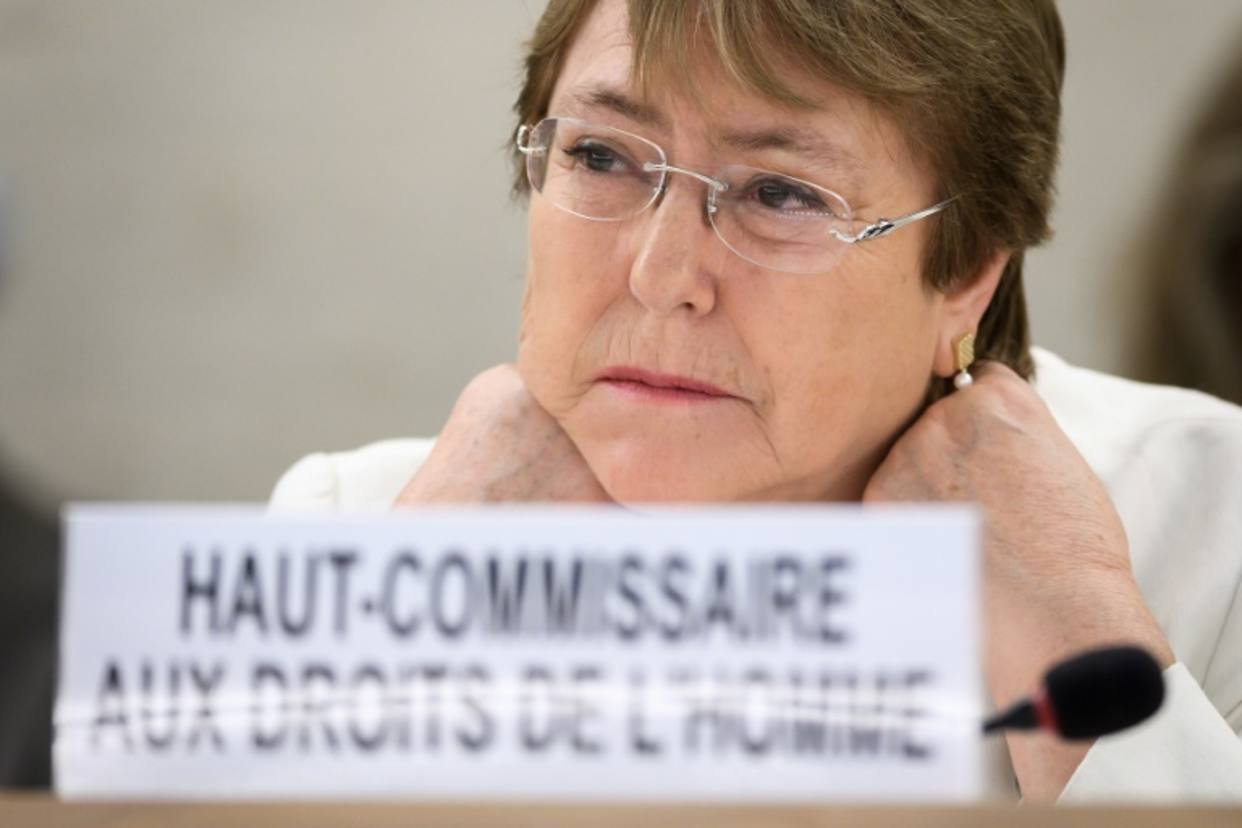
\includegraphics[width=300px]{203.jpg}%
\newline%
%
Michelle Bachelet, alta comisionada de Derechos Humanos de la ONU y ex presidenta de Chile, aceptó reunirse con el canciller de Venezuela, Jorge Arreaza, quien debe pronunciar un discurso este martes ante la organización.%
\newline%
%
Bachelet hizo este lunes su primer discurso frente al Consejo de Derechos Humanos. La alocución, de la que una copia fue transmitida previamente a los medios, contenía párrafos sobre Venezuela, pero la ex presidenta chilena no habló de ello ante los diplomáticos.%
\newline%
%
"Cuando se abre esta sesión, el creciente número de personas que huyen de Venezuela y Nicaragua demuestra una vez más la necesidad de defender constantemente los derechos humanos", indicaba el texto de su discurso.%
\newline%
%
"Es urgente ayudar a los Estados de acogida a resolver los numerosos problemas que provocan estos movimientos", añadía, al tiempo que señalaba que también era importante abordar las razones que provocaban la migración venezolana.%
\newline%
%
Además, Bachelet pedía al Consejo que tomara las medidas disponibles para hacer frente a las violaciones de los derechos humanos tanto en Venezuela como en Nicaragua.%
\newline%
%
Indicaba también que desde la publicación en junio del informe del Alto Comisionado, la instancia siguió recibiendo información sobre violaciones de derechos en el país.%
\newline%
%
\end{document}